% Options for packages loaded elsewhere
\PassOptionsToPackage{unicode}{hyperref}
\PassOptionsToPackage{hyphens}{url}
%
\documentclass[
]{article}
\usepackage{amsmath,amssymb}
\usepackage{iftex}
\ifPDFTeX
  \usepackage[T1]{fontenc}
  \usepackage[utf8]{inputenc}
  \usepackage{textcomp} % provide euro and other symbols
\else % if luatex or xetex
  \usepackage{unicode-math} % this also loads fontspec
  \defaultfontfeatures{Scale=MatchLowercase}
  \defaultfontfeatures[\rmfamily]{Ligatures=TeX,Scale=1}
\fi
\usepackage{lmodern}
\ifPDFTeX\else
  % xetex/luatex font selection
\fi
% Use upquote if available, for straight quotes in verbatim environments
\IfFileExists{upquote.sty}{\usepackage{upquote}}{}
\IfFileExists{microtype.sty}{% use microtype if available
  \usepackage[]{microtype}
  \UseMicrotypeSet[protrusion]{basicmath} % disable protrusion for tt fonts
}{}
\makeatletter
\@ifundefined{KOMAClassName}{% if non-KOMA class
  \IfFileExists{parskip.sty}{%
    \usepackage{parskip}
  }{% else
    \setlength{\parindent}{0pt}
    \setlength{\parskip}{6pt plus 2pt minus 1pt}}
}{% if KOMA class
  \KOMAoptions{parskip=half}}
\makeatother
\usepackage{xcolor}
\usepackage[margin=1in]{geometry}
\usepackage{color}
\usepackage{fancyvrb}
\newcommand{\VerbBar}{|}
\newcommand{\VERB}{\Verb[commandchars=\\\{\}]}
\DefineVerbatimEnvironment{Highlighting}{Verbatim}{commandchars=\\\{\}}
% Add ',fontsize=\small' for more characters per line
\usepackage{framed}
\definecolor{shadecolor}{RGB}{248,248,248}
\newenvironment{Shaded}{\begin{snugshade}}{\end{snugshade}}
\newcommand{\AlertTok}[1]{\textcolor[rgb]{0.94,0.16,0.16}{#1}}
\newcommand{\AnnotationTok}[1]{\textcolor[rgb]{0.56,0.35,0.01}{\textbf{\textit{#1}}}}
\newcommand{\AttributeTok}[1]{\textcolor[rgb]{0.13,0.29,0.53}{#1}}
\newcommand{\BaseNTok}[1]{\textcolor[rgb]{0.00,0.00,0.81}{#1}}
\newcommand{\BuiltInTok}[1]{#1}
\newcommand{\CharTok}[1]{\textcolor[rgb]{0.31,0.60,0.02}{#1}}
\newcommand{\CommentTok}[1]{\textcolor[rgb]{0.56,0.35,0.01}{\textit{#1}}}
\newcommand{\CommentVarTok}[1]{\textcolor[rgb]{0.56,0.35,0.01}{\textbf{\textit{#1}}}}
\newcommand{\ConstantTok}[1]{\textcolor[rgb]{0.56,0.35,0.01}{#1}}
\newcommand{\ControlFlowTok}[1]{\textcolor[rgb]{0.13,0.29,0.53}{\textbf{#1}}}
\newcommand{\DataTypeTok}[1]{\textcolor[rgb]{0.13,0.29,0.53}{#1}}
\newcommand{\DecValTok}[1]{\textcolor[rgb]{0.00,0.00,0.81}{#1}}
\newcommand{\DocumentationTok}[1]{\textcolor[rgb]{0.56,0.35,0.01}{\textbf{\textit{#1}}}}
\newcommand{\ErrorTok}[1]{\textcolor[rgb]{0.64,0.00,0.00}{\textbf{#1}}}
\newcommand{\ExtensionTok}[1]{#1}
\newcommand{\FloatTok}[1]{\textcolor[rgb]{0.00,0.00,0.81}{#1}}
\newcommand{\FunctionTok}[1]{\textcolor[rgb]{0.13,0.29,0.53}{\textbf{#1}}}
\newcommand{\ImportTok}[1]{#1}
\newcommand{\InformationTok}[1]{\textcolor[rgb]{0.56,0.35,0.01}{\textbf{\textit{#1}}}}
\newcommand{\KeywordTok}[1]{\textcolor[rgb]{0.13,0.29,0.53}{\textbf{#1}}}
\newcommand{\NormalTok}[1]{#1}
\newcommand{\OperatorTok}[1]{\textcolor[rgb]{0.81,0.36,0.00}{\textbf{#1}}}
\newcommand{\OtherTok}[1]{\textcolor[rgb]{0.56,0.35,0.01}{#1}}
\newcommand{\PreprocessorTok}[1]{\textcolor[rgb]{0.56,0.35,0.01}{\textit{#1}}}
\newcommand{\RegionMarkerTok}[1]{#1}
\newcommand{\SpecialCharTok}[1]{\textcolor[rgb]{0.81,0.36,0.00}{\textbf{#1}}}
\newcommand{\SpecialStringTok}[1]{\textcolor[rgb]{0.31,0.60,0.02}{#1}}
\newcommand{\StringTok}[1]{\textcolor[rgb]{0.31,0.60,0.02}{#1}}
\newcommand{\VariableTok}[1]{\textcolor[rgb]{0.00,0.00,0.00}{#1}}
\newcommand{\VerbatimStringTok}[1]{\textcolor[rgb]{0.31,0.60,0.02}{#1}}
\newcommand{\WarningTok}[1]{\textcolor[rgb]{0.56,0.35,0.01}{\textbf{\textit{#1}}}}
\usepackage{graphicx}
\makeatletter
\def\maxwidth{\ifdim\Gin@nat@width>\linewidth\linewidth\else\Gin@nat@width\fi}
\def\maxheight{\ifdim\Gin@nat@height>\textheight\textheight\else\Gin@nat@height\fi}
\makeatother
% Scale images if necessary, so that they will not overflow the page
% margins by default, and it is still possible to overwrite the defaults
% using explicit options in \includegraphics[width, height, ...]{}
\setkeys{Gin}{width=\maxwidth,height=\maxheight,keepaspectratio}
% Set default figure placement to htbp
\makeatletter
\def\fps@figure{htbp}
\makeatother
\setlength{\emergencystretch}{3em} % prevent overfull lines
\providecommand{\tightlist}{%
  \setlength{\itemsep}{0pt}\setlength{\parskip}{0pt}}
\setcounter{secnumdepth}{-\maxdimen} % remove section numbering
\ifLuaTeX
  \usepackage{selnolig}  % disable illegal ligatures
\fi
\IfFileExists{bookmark.sty}{\usepackage{bookmark}}{\usepackage{hyperref}}
\IfFileExists{xurl.sty}{\usepackage{xurl}}{} % add URL line breaks if available
\urlstyle{same}
\hypersetup{
  pdftitle={First Steps in R},
  pdfauthor={Ralf Becker},
  hidelinks,
  pdfcreator={LaTeX via pandoc}}

\title{First Steps in R}
\author{Ralf Becker}
\date{October 2023}

\begin{document}
\maketitle

\hypertarget{learning-outcomes}{%
\section{Learning Outcomes}\label{learning-outcomes}}

This document is for you to experience some very basic functionality in
R/RStudio.

In particular this is for you

\begin{itemize}
\tightlist
\item
  to explore the RStudio interface
\item
  to learn how to search for help
\item
  to not be scared by error messages
\item
  to know how to load libraries
\item
  to upload a datafile
\item
  to explore the contents of this datafile
\item
  to learn what functions do
\item
  to learn about data types
\item
  to undertake some basic data manipulation
\end{itemize}

This Data Lab assumes that you have R and RStudio installed on your
computer. Alternatively you can get yourself an RStudio/Posit Cloud
account (\url{https://posit.cloud/}). The free account is sufficient to
get started. But in the end you should attempt to have RStudio up and
running on your computer.

\hypertarget{prepare-your-workspace}{%
\section{Prepare your Workspace}\label{prepare-your-workspace}}

Before you start you should create a space (i.e.~a folder) on your
computer from where you are planning to do all your R work. Make sure
you understand where that folder is and that you know the path to that
folder.

Let's say you named your folder \texttt{Rwork} on your C drive, then the
path to your folder will be \texttt{C:\textbackslash{}Rwork}.

For this computer lab we are using the datafile
\href{https://datasquad.github.io/ECLR/Data/STATS19_GM_AccData.csv}{STATS19\_GM\_AccData.csv}.
You should download this datafile into the folder you just created and
want to work from. It will also be useful to have the
\href{https://assets.publishing.service.gov.uk/government/uploads/system/uploads/attachment_data/file/995422/stats19.pdf}{Data
Dictionary} ready.

\hypertarget{exploring-rstudio-and-searching}{%
\section{Exploring RStudio and
searching}\label{exploring-rstudio-and-searching}}

RStudio is a software which makes working with the actual statistical
software R easier. In fact, once you followed the installation advice
and have R and RStudio installed, you will never really have to worry
about R anymore. Just start RStudio.

When you load RStudio for the first time you should see something like
this.

\begin{figure}
\centering
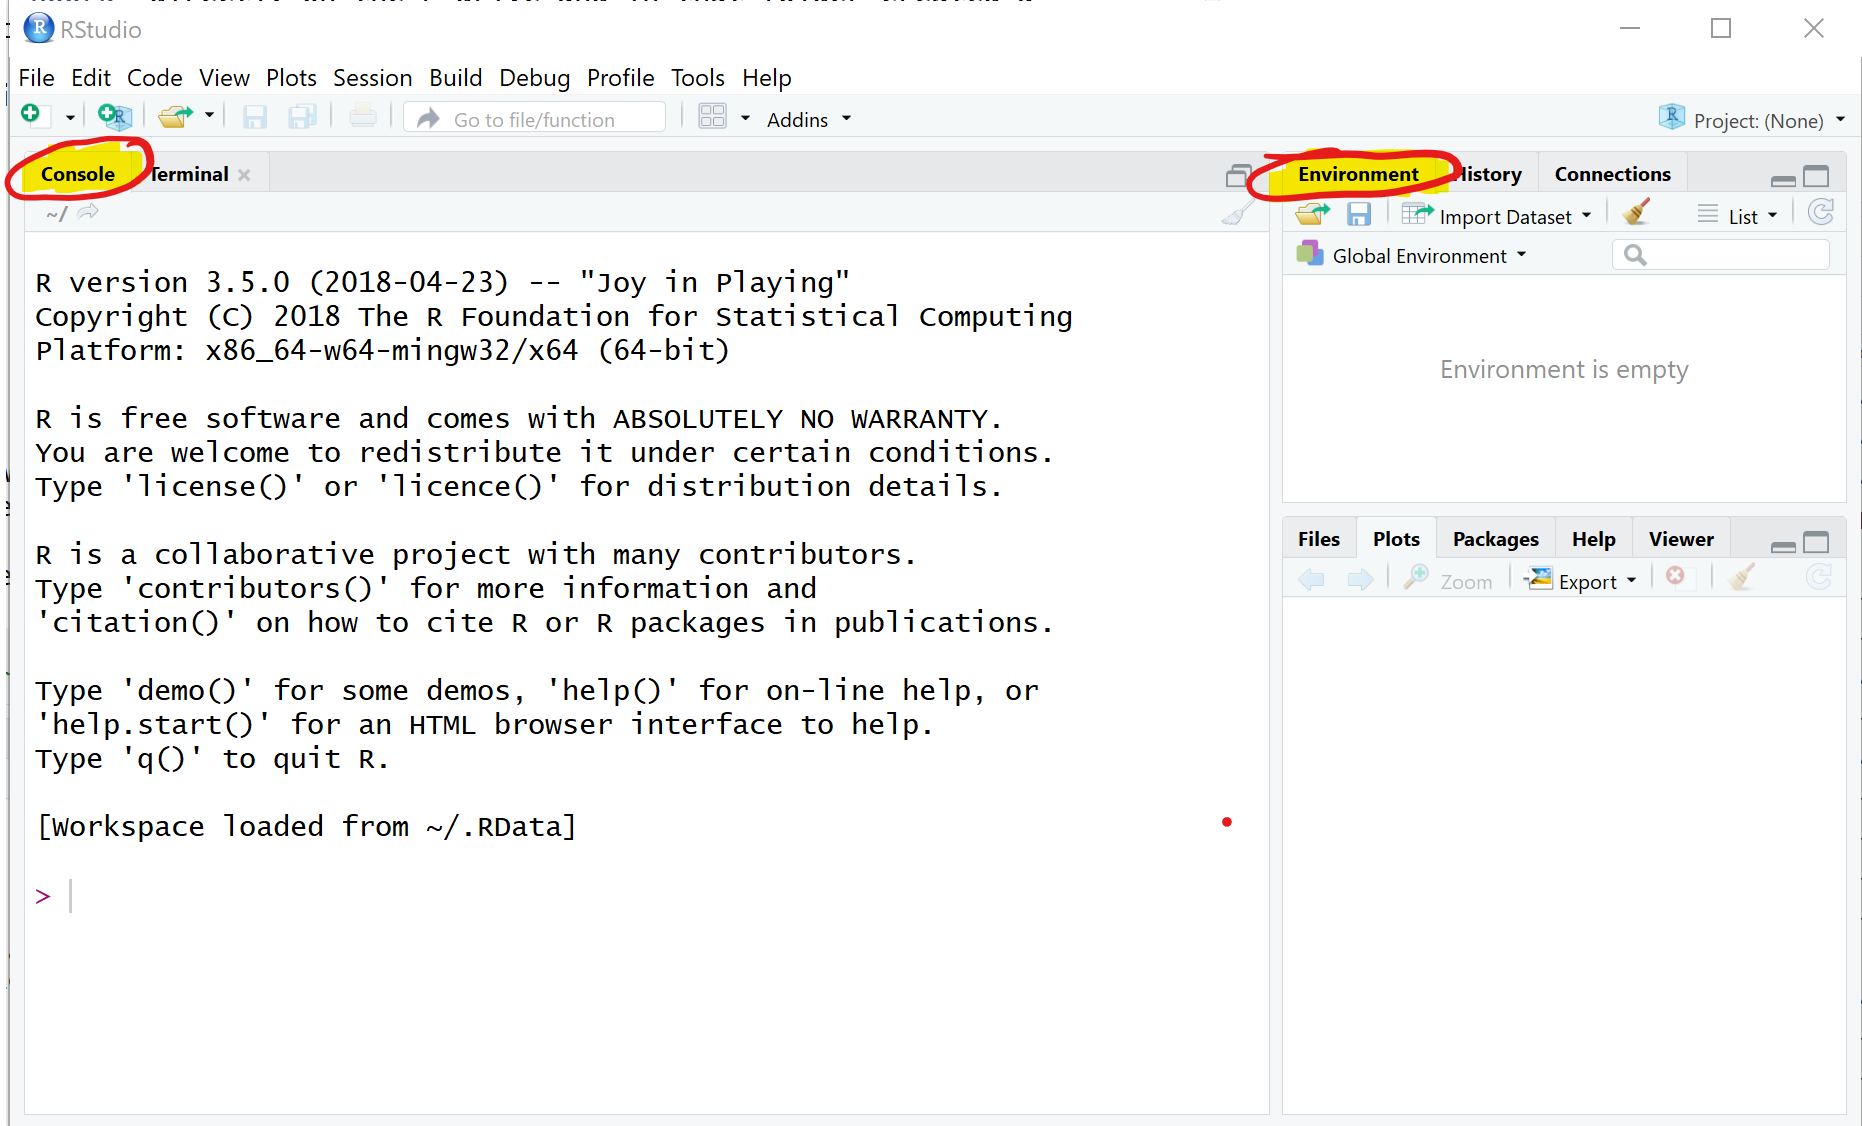
\includegraphics{images/RStudio_image0.png}
\caption{RStudio when loading for the first time}
\end{figure}

There are two important areas on that screen, the Console and the
Environment. The Console is something like your main computational area.
In there you can see some information but at the end an
``\textgreater{}''. This indicates that RStudio is standing ready to do
whatever you want it to do.

Say you want to calculate 3+4 \ldots{} yes, trivial but let's start
small. Type 3+4 into the console (behind the ``\textgreater{}'' sign)
and press enter. Yes you should see the correct result.

\begin{Shaded}
\begin{Highlighting}[]
\DecValTok{3}\SpecialCharTok{+}\DecValTok{4}
\end{Highlighting}
\end{Shaded}

\begin{verbatim}
## [1] 7
\end{verbatim}

That was easy, let's see whether you can get R to calculate \(13^2\),
\(\sqrt{7569}\), \(e^{5}\) and \(ln(5)\). The first you achieve as
follows:

\begin{Shaded}
\begin{Highlighting}[]
\DecValTok{13}\SpecialCharTok{\^{}}\DecValTok{2}
\end{Highlighting}
\end{Shaded}

\begin{verbatim}
## [1] 169
\end{verbatim}

What about the others. Well, at this stage we will introduce you to two
of the most inportant programming techniques there are:

\begin{enumerate}
\def\labelenumi{\arabic{enumi}.}
\tightlist
\item
  Just try it. Do you have a hunch how to do it? Test it. I am yet to
  hear that someone broke their computer by entering an incorrect
  command in RStudio.
\item
  searching on the Web (say in Google, Bing, Baidu or DuckDuckGo)! For
  instance if you want to know how to calculate a square root in R you
  may want to search for ``how to calculate a square root in R'' and you
  should find the appropriate advice. Practice your search technique to
  calculate the above solutions. Check against your calculator.
\end{enumerate}

\hypertarget{functions}{%
\section{Functions}\label{functions}}

Functions are important building blocks of any programming language. You
just used your first function. Hopefully you found out that the way to
calculate \(\sqrt{7569}\) was to type

\begin{Shaded}
\begin{Highlighting}[]
\FunctionTok{sqrt}\NormalTok{(}\DecValTok{7569}\NormalTok{)}
\end{Highlighting}
\end{Shaded}

\begin{verbatim}
## [1] 87
\end{verbatim}

Giving you the result 87. What you used here is a function, namely the
\texttt{sqrt} function which some clever programmer wrote in order to
calculate a square root. The anatomy of a function is
\texttt{function\_name(input)}. Think of a function as a drink machine.

\begin{figure}
\centering
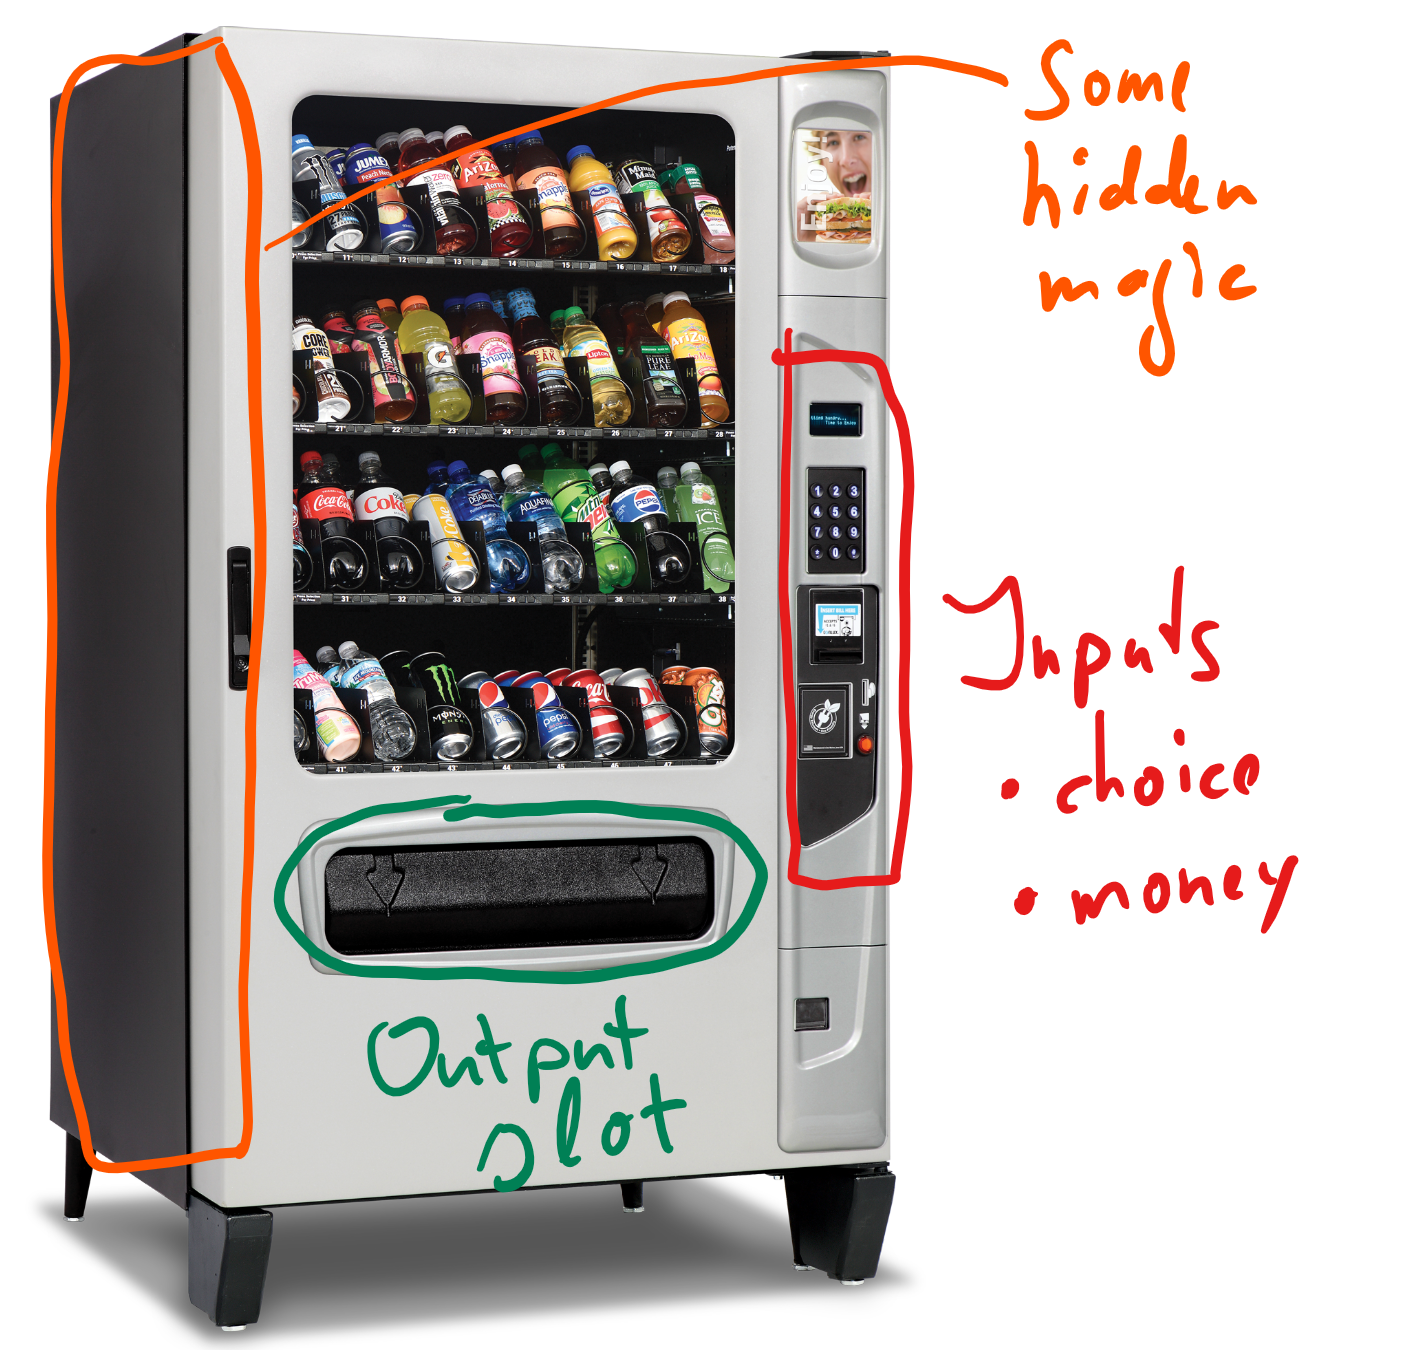
\includegraphics[width=0.5\textwidth,height=\textheight]{images/DrinkMachine.png}
\caption{A drink machine is a function.}
\end{figure}

Most functions require some input. Our function, the \texttt{sqrt}
function needs a number of which to take the square root. The output in
our example, 87, is then returned. In our case it is returned to be
printed in the Console window.

\hypertarget{creating-variables}{%
\section{Creating variables}\label{creating-variables}}

So far you have learned that R can be used as a glorified calculator.
Let's start to explore why R is way more powerful that that. You can
save the results of as many calculations as you want and you can easily
reuse the results of some calculations in later calculations.

Type ``a\textless-12/4'' into the console (without the quotation marks)
and press enter

\begin{Shaded}
\begin{Highlighting}[]
\NormalTok{a }\OtherTok{\textless{}{-}} \DecValTok{12}\SpecialCharTok{/}\DecValTok{4}
\end{Highlighting}
\end{Shaded}

You will see that in the console the correct result does not show, but
in the Environment pane of your RStudio window you should now see an
entry

\begin{figure}
\centering
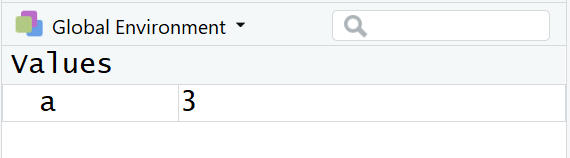
\includegraphics{images/RStudio_Env.png}
\caption{RStudio Environment saves variables}
\end{figure}

What did the command ``a\textless-12/4'' actually do? In words:
``Calculate 12/4 and assign (\textless-) the result to a variable called
\texttt{a}.''

With that in mind implement the following: ``Calculate 11*11 and assign
(\textless-) the result to a variable called \texttt{A}.''

You should now see two variables in your Environment pane. Let's add
another: ``Calculate the square root of 64 and assign (\textless-) the
result to a variable called \texttt{b}.''

Note that we used the \texttt{sqrt} function again, but this time the
output was not send to be printed in the Console, but instead it was
send to the new variable \texttt{b}. If you have done everything right
your Environment panel should now look as follows

\begin{figure}
\centering
\includegraphics{RStudio_Env2.png}
\caption{RStudio Environment saves variables}
\end{figure}

Note that \texttt{a} and \texttt{A} are different variables, so R is
case-sensitive! All the variables listed in the Environment can be
re-used for further calculations. For example:

\begin{Shaded}
\begin{Highlighting}[]
\NormalTok{d }\OtherTok{\textless{}{-}}\NormalTok{ A }\SpecialCharTok{{-}}\NormalTok{ a }\SpecialCharTok{+} \DecValTok{2}\SpecialCharTok{*}\NormalTok{b}
\end{Highlighting}
\end{Shaded}

Let's perform another calculation in which we use the result of the last
calculation:

\begin{Shaded}
\begin{Highlighting}[]
\NormalTok{e }\OtherTok{\textless{}{-}}\NormalTok{ D }\SpecialCharTok{{-}} \DecValTok{3}\SpecialCharTok{*}\NormalTok{a}
\end{Highlighting}
\end{Shaded}

\begin{verbatim}
## Error in D - 3 * a: non-numeric argument to binary operator
\end{verbatim}

You will see R throwing an error message at you: ``Error in D - 3 * a :
non-numeric argument to binary operator''. Ehmmm \ldots{} what does this
mean? Actually not a lot. In the first instance this tells you that
something went wrong in that command. Can you see what the problem is?
Remember R is trying to perform the calculation to the right of
\texttt{\textless{}-} and then assign this to a new variable \texttt{e}.
Does it have all the info on the right hand side? Check your list of
variables in the Environment panel. Recall that R is case sensitive.

An important lesson with respect to error messages

\begin{itemize}
\tightlist
\item
  You will see them ALL THE TIME, and that is fine
\item
  You cannot break the computer with any errors in R, so don't worry,
  just try.
\item
  Re-read what you typed, is it actually what you wanted to do.
\item
  Read the error message. Sometimes it will give you a clue as to what
  the problem is \ldots{} unfortunately not here!
\end{itemize}

\begin{center}\rule{0.5\linewidth}{0.5pt}\end{center}

So, we have done a bit of work so far. Let's take a short break. Please
close RStudio and click ``Don't Save'' when you get the message in the
next image.

\begin{figure}
\centering
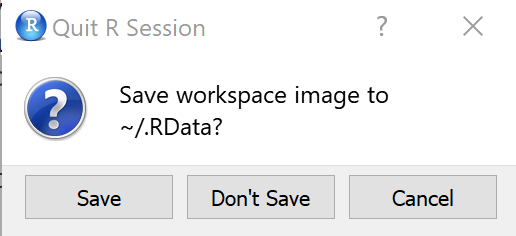
\includegraphics{images/RStudio_SaveWorkspace.png}
\caption{RStudio Environment saves variables}
\end{figure}

Get up, stretch your legs and get yourself a glass to drink. Then come
back and open RStudio again so that we can continue our work.

As you open you should get exactly the same initial layout as before
\ldots{} What value did \texttt{e} have again???? (125 if you managed to
correct the above error) Where are our calculations??? Unless you worked
in a script file, all your work is gone now. The next section is to
teach you the right workflow such that this does not happen with your
important work.

\hypertarget{preparing-your-script-file-and-libraries}{%
\section{Preparing your script file and
libraries}\label{preparing-your-script-file-and-libraries}}

For all significant work you want to make sure that you save the work
you have done, such that you do not have to re-type things which you did
yesterday \ldots{} or just before I asked you to get a glass of water.
The way to ensure that is to save all your work in a script file. A
script file is basically a text file which saves all your commands (and
comments - see below) and from where RStudio can easily execute these
commands.

Let's create a script file. Via the RStudio menu (FILE - NEW FILE - R
SCRIPT) open a new script file and safe it in the folder from which you
want to work (see above).

Start by creating a comment line at the top of that file which may say
something like

\begin{Shaded}
\begin{Highlighting}[]
\CommentTok{\# File for first SE Data Lab}
\CommentTok{\# October 2023}
\CommentTok{\# exciting!!!}
\end{Highlighting}
\end{Shaded}

\begin{quote}
Note: Adding comments to your code is absolutely vital if you want to
understand tomorrow what you did today. I am not joking, adding comments
to explain to your future self what you are doing is absolutly critical.
Everything which follows the \texttt{\#} sign is a comment and is
effectively ignored by R. It is written not for R but for your future
self!
\end{quote}

If not mentioned otherwise all the following code should be added to
that script file and executed from there. Save that file and make sure
you know where you save it as, next week, you may want to continue to
work on this.

Next, you should ensure that you set the working directory to the
directory where your scriptfile and datafile is in. If your folder was
\texttt{C:\textbackslash{}Rwork} then the command below should read
\texttt{setwd("C:/Rwork")}. Note that all backward slashes
(\texttt{\textbackslash{}}) have to be replaced by forward slashes
(\texttt{/}). Don't ask why, just accept ;-).

\begin{Shaded}
\begin{Highlighting}[]
\FunctionTok{setwd}\NormalTok{(}\StringTok{"XXXX:/XXXX"}\NormalTok{)   }\CommentTok{\# replace the XXXX with your drive and path}
\end{Highlighting}
\end{Shaded}

\begin{quote}
Note; If you are having trouble finding the location of your script
file, or how to formally write it down, this is a trick. In the menu to
RStudio click on teh following: ``Session'' - ``Set Working Directory''
- ``To Source File Location''. RStudio will find the path to your script
and will execute the command. You can then copy the command from the
console into your script such that you have it saved for next time.
\end{quote}

Load the libraries which we want to use.

\begin{Shaded}
\begin{Highlighting}[]
\FunctionTok{library}\NormalTok{(tidyverse)    }\CommentTok{\# for almost all data handling tasks}
\FunctionTok{library}\NormalTok{(ggplot2)      }\CommentTok{\# to produce nice graphiscs}
\end{Highlighting}
\end{Shaded}

\begin{quote}
Note: Libraries are collections of functions which add great
functionality. They are not included in the base R installation and
hence need to be added to your computer (see installation advice for
packages below - this only has to be done once on each computer).
However, even once they are installed on you need to make this new
functionality available to your code. This is what the \texttt{library}
functions do. This has to be done at the beginning of every script file
in which you want to use the respective functionality.
\end{quote}

By just typing these commands into the script file nothing is actually
happening. If you want R to execute any of the commands in your script
file you have to do one of the following:

\begin{figure}
\centering
\includegraphics{images/RStudio_Image1.png}
\caption{RStudio Environment saves variables}
\end{figure}

\begin{enumerate}
\def\labelenumi{\arabic{enumi}.}
\tightlist
\item
  Press the ``Source'' button, in which case R will execute all commands
  in the script file
\item
  Press the ``Run'' button, in which case R will run the command in
  which the curser currently is
\item
  Press the ``CTRL''+``ENTER'' on the keyboard (COMMAND + ENTER on a
  mac), in which case R will run the command in which the curser
  currently is
\item
  Highlight several lines and press ``CTRL''+``ENTER'' on the keyboard
  (COMMAND + ENTER on a mac), in which case R will run the commands in
  the highlighted lines
\end{enumerate}

If RStudio tells you that one or more of these libraries are not
installed then install these (not any others) on the machine you are
working from. For instance, if \texttt{ggplot2} was not installed you
would receive an error message like ``Error in library(ggplot2) : there
is no package called `ggplot2'\,'', and in that case you should run:

\begin{Shaded}
\begin{Highlighting}[]
\FunctionTok{install.packages}\NormalTok{(}\StringTok{"ggplot2"}\NormalTok{)}
\end{Highlighting}
\end{Shaded}

You can run this straight from the command/console or you could instead
install the package via the packages tab on the right hand side. You
will need to do this only once on your computer and once you have done
that you can call \texttt{library(ggplot2)} again without running into
problems.

\hypertarget{data-upload}{%
\section{Data Upload}\label{data-upload}}

Make sure you have set the working directory to the directory in which
you saved your script file and the data file (see above). As we are
dealing with data in a csv file we will use the \texttt{read.csv}
function to load the data. We are lucky that this datafile has no
missing data, meaning that it has no empty cells. Missing information
all appear to be coded up as a special category in each of the
variables. See the
\href{https://assets.publishing.service.gov.uk/government/uploads/system/uploads/attachment_data/file/995422/stats19.pdf}{Data
Dictionary} to confirm that for the \texttt{RoadType} variable a 9
represents ``Unknown''.

\begin{Shaded}
\begin{Highlighting}[]
\NormalTok{accdata }\OtherTok{\textless{}{-}} \FunctionTok{read.csv}\NormalTok{(}\StringTok{"STATS19\_GM\_AccData.csv"}\NormalTok{)}
\end{Highlighting}
\end{Shaded}

It is well possible that you receive the following error message as you
execute this command ``Error: \texttt{path} does not exist:
`STATS19\_GM\_AccData.csv'\,''. The most likely reason for this is that
the ``STATS19\_GM\_AccData.csv'' is not saved in your working directory.
Make sure you download that file from Blackboard and save it in the
working directory you created earlier and you used in the
\texttt{setwd()} command. Also make sure that the file name used in the
command here matches exactly the file name in your folder.

Make sure that your data upload is successful. You should see an object
\texttt{accdata} in your environment. You can also run the \texttt{str}
(structure) function.

\begin{Shaded}
\begin{Highlighting}[]
\FunctionTok{str}\NormalTok{(accdata)  }\CommentTok{\# prints some basic info on variables}
\end{Highlighting}
\end{Shaded}

\begin{verbatim}
## 'data.frame':    42624 obs. of  27 variables:
##  $ Accident.Index               : num  102262412010 102262562010 102264322010 107264182010 114261842010 ...
##  $ Year                         : int  2010 2010 2010 2010 2010 2010 2010 2010 2010 2010 ...
##  $ Severity                     : int  3 3 3 3 3 3 3 3 3 3 ...
##  $ NumberVehicles               : int  2 2 2 3 1 1 1 2 2 1 ...
##  $ NumberCasualties             : int  1 1 1 1 1 1 1 1 1 1 ...
##  $ OutputDate                   : chr  "01/01/2010" "01/01/2010" "01/01/2010" "01/01/2010" ...
##  $ Day                          : int  6 6 6 6 6 6 7 7 7 7 ...
##  $ OutputTime                   : chr  "13:10" "11:10" "17:30" "13:49" ...
##  $ Easting                      : int  382347 381892 385840 377762 355982 362380 365767 381775 383868 384681 ...
##  $ Northing                     : int  390025 390582 403134 403302 404620 407476 405672 410735 394065 395127 ...
##  $ LocalAuthority               : int  102 102 102 107 114 114 100 101 102 102 ...
##  $ Road1Class                   : int  5 7 4 4 4 5 4 5 4 6 ...
##  $ Road1Number                  : int  5166 0 664 666 577 5239 58 6221 5103 0 ...
##  $ CarriagewayType              : int  3 6 3 3 6 6 6 6 3 6 ...
##  $ SpeedLimit                   : int  50 30 30 30 30 30 30 30 40 30 ...
##  $ JunctionDetail               : int  6 3 3 3 0 0 3 3 6 3 ...
##  $ JunctionControl              : int  2 4 4 4 0 0 2 4 2 4 ...
##  $ Road2Class                   : int  3 7 7 1 0 0 5 7 4 7 ...
##  $ Road2Number                  : int  5103 0 0 60 0 0 5235 0 6010 0 ...
##  $ PedCrossingHumanControl      : int  0 0 0 0 0 0 0 0 0 0 ...
##  $ PedCrossingPhysicalFacilities: int  0 0 0 0 0 0 5 0 5 0 ...
##  $ LightingCondition            : int  1 1 4 3 7 4 4 1 4 4 ...
##  $ WeatherCondition             : int  1 1 1 9 9 1 1 3 3 8 ...
##  $ RoadSurface                  : int  4 4 2 1 1 4 4 3 2 4 ...
##  $ SpecialConditions            : int  0 0 0 0 0 0 0 0 0 0 ...
##  $ CarriagewayHazard            : int  0 0 0 0 0 0 0 0 0 0 ...
##  $ PlaceReported                : int  1 1 2 2 2 1 1 2 1 1 ...
\end{verbatim}

You should now see the \texttt{accdata} object in your Environment
(right hand pane).

There are 42,624 observations, each representing one recorded accident
in Greater Manchester (GM) between 2010 and 2020. Each accident has
variables which characterise the accident.

The following variables will be important for the analysis here:

\begin{itemize}
\tightlist
\item
  \texttt{Accident.Index}, this is a unique identifier for each accident
\item
  \texttt{Year}, gives the year in which the accident happened
\item
  \texttt{Severity}, a variable coding the severity of the accident,
  although we are unsure how this is coded
\item
  \texttt{NumberVehicles}, number of vehicles involved in the accident
\item
  \texttt{NumberCasualties}, number of casualties involved in the
  accident
\item
  \texttt{LightingCondition}, Lighting conditions at time and location
  of accident
\item
  \texttt{WeatherCondition}, Weather conditions at time and location of
  accident
\item
  \texttt{Road1Class}, lower numbers indicating more major roads, 1 =
  Motorway
\item
  \texttt{RoadSurface}, indicator of whether the road surface was dry
  wet or icy at the time and place of the accident
\end{itemize}

You wrote your first script. It is time to have another break. Make sure
you save your script and then close RStudio (you don't need to do that
in general, but please do it at this point to help me demonstrate the
value of scripts). After relaxing for a few minutes and telling your
flatmate that you are on your way to become an expert data analyst, come
back and re-open RStudio. Load the script file (if it wasn't loaded
automatically). The environment should, at this stage be empty, but if
you click on the ``Source'' button then R will automatically execute all
the commands you had in your script and \texttt{accdata} should be
available in the Environment panel.

So that is the value of scripts! You can easily pick up where you left
your work, no need to redo anything.

\hypertarget{accessing-data}{%
\section{Accessing data}\label{accessing-data}}

The \texttt{accdata} item in your environment basically contains the
entire spreadsheet of data. You can look at the entire spreadsheet by
clicking on the tiny spreadsheet in the \texttt{accdata} line. This will
open a new tab with the spreadsheet. Have a look and then close the tab
again.

It is important to know how you can access subsets of data. Run through
the following commands to see what happens. Perhaps also experiment a
bit by changing the commands and predicting what the outcome should be.

\begin{Shaded}
\begin{Highlighting}[]
\NormalTok{accdata[}\DecValTok{1}\NormalTok{,]}
\NormalTok{accdata[,}\DecValTok{2}\NormalTok{]}
\NormalTok{accdata[}\DecValTok{3}\NormalTok{,}\DecValTok{4}\NormalTok{]}
\NormalTok{accdata[,}\DecValTok{4}\SpecialCharTok{:}\DecValTok{6}\NormalTok{]}
\NormalTok{accdata[}\DecValTok{4}\SpecialCharTok{:}\DecValTok{6}\NormalTok{]}
\NormalTok{accdata[}\DecValTok{2}\SpecialCharTok{:}\DecValTok{4}\NormalTok{,}\DecValTok{5}\SpecialCharTok{:}\DecValTok{10}\NormalTok{]}
\NormalTok{accdata}\SpecialCharTok{$}\NormalTok{SpeedLimit}
\NormalTok{accdata}\SpecialCharTok{$}\NormalTok{SpeedLimit[}\DecValTok{1}\SpecialCharTok{:}\DecValTok{5}\NormalTok{]}
\NormalTok{accdata[}\FunctionTok{c}\NormalTok{(}\StringTok{"SpeedLimit"}\NormalTok{,}\StringTok{"Road1Class"}\NormalTok{)]}
\end{Highlighting}
\end{Shaded}

These are all different ways to select particular observations (rows in
a spreadsheet) and variables (columns in a spreadsheet). There were two
particular techniques which are important

\begin{itemize}
\tightlist
\item
  \texttt{accdata\$SpeedLimit} did address the \texttt{SpeedLimit}
  variable in the \texttt{accdata} dataset (\texttt{DATASET\$VARIABLE}).
\item
  \texttt{c("SpeedLimit","Road1Class")} allowed us to access two very
  particular variables, ignoring all other 25 variables. It is useful to
  know what \texttt{c("SpeedLimit","Road1Class")} actually does.
\end{itemize}

\begin{Shaded}
\begin{Highlighting}[]
\FunctionTok{c}\NormalTok{(}\StringTok{"SpeedLimit"}\NormalTok{,}\StringTok{"Road1Class"}\NormalTok{)}
\end{Highlighting}
\end{Shaded}

\begin{verbatim}
## [1] "SpeedLimit" "Road1Class"
\end{verbatim}

It creates a list with two elements, here two text strings. But you can
also create lists with numbers.

\begin{Shaded}
\begin{Highlighting}[]
\FunctionTok{c}\NormalTok{(}\FloatTok{3.5}\NormalTok{,}\DecValTok{2}\SpecialCharTok{/}\DecValTok{3}\NormalTok{)}
\end{Highlighting}
\end{Shaded}

\begin{verbatim}
## [1] 3.50 0.67
\end{verbatim}

In fact you could even create lists which mixed datatypes.

\begin{Shaded}
\begin{Highlighting}[]
\FunctionTok{c}\NormalTok{(}\StringTok{"Countries in the EU"}\NormalTok{, }\DecValTok{28{-}1}\NormalTok{, }\StringTok{":{-}("}\NormalTok{)}
\end{Highlighting}
\end{Shaded}

\begin{verbatim}
## [1] "Countries in the EU" "27"                  ":-("
\end{verbatim}

Lists are quite fundamental to the way how R stores data. If you
assigned any of the above to a variable, for instance

\begin{Shaded}
\begin{Highlighting}[]
\NormalTok{silly\_list }\OtherTok{\textless{}{-}} \FunctionTok{c}\NormalTok{(}\StringTok{"Countries in the EU"}\NormalTok{, }\DecValTok{28{-}1}\NormalTok{, }\StringTok{":{-}("}\NormalTok{)}
\end{Highlighting}
\end{Shaded}

you would have saved it in the Environment and could re-use it.

All the commands in this section were really only to explore the
functionality of R. There is no need to save these in your script file.
But no harm either as none of these actually changed the values of the
data in \texttt{accdata}.

\hypertarget{do-not-change-your-original-data-sheet-here-the-csv-file}{%
\section{Do not change your original data sheet (here the csv
file)}\label{do-not-change-your-original-data-sheet-here-the-csv-file}}

An important principle of working with data here is that you should
never change your original datafile, which in this case the
\texttt{STATS19\_GM\_AccData.csv} file. As you can see from our work so
far we merely upload the csv file and then use the data here in R, but
we will not go back to the original csv file and change anything in
there. And that is very important. In that way you can always start
again with your analysis from your original data.

If you were to make any changes in your csv file, these changes would be
irreversible.

\hypertarget{investigate-data-1}{%
\section{Investigate Data 1}\label{investigate-data-1}}

Let's find out how the severity of an accident is coded like. If you
wish to find out what different values the variable takes in your
dataset you can easily see that with:

\begin{Shaded}
\begin{Highlighting}[]
\FunctionTok{unique}\NormalTok{(accdata}\SpecialCharTok{$}\NormalTok{Severity)}
\end{Highlighting}
\end{Shaded}

\begin{verbatim}
## [1] 3 2 1
\end{verbatim}

But what do the values 1, 2 or 3 represent?

The usual advice would be to go to the data dictionary and check the
coding, but all we can see on the data entry form is the following

\begin{figure}
\centering

\includegraphics[width=0.5\textwidth,height=\textheight]{images/serious.png}
\caption{Seriousness info}
\end{figure}

But does a 1 in the \texttt{Severity} variable indicate a fatal or a
slight accident. We will have to check from the data itself. I am sure
you could come up with different ways of checking.

Presumably there will be mostly slight accidents and very few fatal
ones. So if we look up the number of accidents in each category it seems
reasonable to assume that the category with the largest number of
observations is the slight one.

The easiest way to look at this is to use the \texttt{table} function on
the \texttt{Severity} variable

\begin{Shaded}
\begin{Highlighting}[]
\FunctionTok{table}\NormalTok{(accdata}\SpecialCharTok{$}\NormalTok{Severity)}
\end{Highlighting}
\end{Shaded}

\begin{verbatim}
## 
##     1     2     3 
##   582  6519 35523
\end{verbatim}

Judging from here it is apparent that category 1 is likely to be the
severe accident category and category 3 the slight one.

\hypertarget{data-formats}{%
\section{Data Formats}\label{data-formats}}

We can see (from the output to \texttt{str(accdata)}) that almost all
variables are integer (\texttt{int}) variables, i.e.~the software will
treat them as whole numbers. Only the date and time variables are text
(character, \texttt{chr}) variables and the \texttt{AAcidentIndex} is a
\texttt{num} variable. Also numeric but not restricted to whole numbers
like \texttt{int}.

Recall that for most of the variables the numbers actually represent
categories. Like for the \texttt{Severity} variable where we previously
established that 1 = fatal, 2 = serious and 3 = slight. For later it
will be convenient to have \texttt{Severity} coded as a variable which
is not numeric, but a categorical variables. In other words a variable
which recognises that there are only limited possible outcomes (here 3).

In R such variables are called \texttt{factor} variables. Hence we will
create a new variables, \texttt{Severityf} which contains the same info,
but just in a way easier to understand.

\begin{Shaded}
\begin{Highlighting}[]
\NormalTok{accdata}\SpecialCharTok{$}\NormalTok{Severityf }\OtherTok{\textless{}{-}} \FunctionTok{as.factor}\NormalTok{(accdata}\SpecialCharTok{$}\NormalTok{Severity)  }\CommentTok{\# translates a variable into a factor variable}
\FunctionTok{levels}\NormalTok{(accdata}\SpecialCharTok{$}\NormalTok{Severityf) }\OtherTok{\textless{}{-}} \FunctionTok{c}\NormalTok{(}\StringTok{"Fatal"}\NormalTok{,}\StringTok{"Serious"}\NormalTok{,}\StringTok{"Slight"}\NormalTok{) }\CommentTok{\# changes the names of the categories}
\FunctionTok{table}\NormalTok{(accdata}\SpecialCharTok{$}\NormalTok{Severityf)}
\end{Highlighting}
\end{Shaded}

\begin{verbatim}
## 
##   Fatal Serious  Slight 
##     582    6519   35523
\end{verbatim}

There are a number of important elements in these lines

\begin{itemize}
\tightlist
\item
  \texttt{accdata\$Severityf\ \textless{}-} creates a new variable in
  the \texttt{accdata} object, called \texttt{Severityf}.
  \texttt{\textless{}-} is called the assignment operator and it assigns
  some value to that new variable. It will assign whatever comes to the
  right hand side of \texttt{\textless{}-}
\item
  \texttt{as.factor()} is a function called \texttt{as.factor}. If you
  want to find out what a function does you can call the help function
  \texttt{?as.factor}. This one creates a variable as a factor
  (categorical) variable. But it requires an input (Whatever comes
  inside the parenthesis). Here we ask R to use the variable
  \texttt{accdata\$Severity} to create a new factor variable
  (\texttt{Severity} itself is an \texttt{int} variable).
\item
  \texttt{levels(accdata\$Severityf)\ \textless{}-\ c("Fatal","Serious","Slight")}
  then changes the names of the levels (categories) into sensible names.
  Here we use again the assignment operator \texttt{\textless{}-}. The
  order matters, but we learn from the earlier analysis that: 1 = fatal,
  2 = serious and 3 = slight. As \texttt{Severity} is a numerical
  (\texttt{int}) variable it will order the categories in numerical
  order, 1 first and 3 last. In doubt you will have to check that you
  have used the right ordering by comparing the \texttt{Severity} and
  \texttt{Severityf} variable.
\end{itemize}

Now create two new variables \texttt{WeatherConditionf} and
\texttt{RoadSurfacef} which achieve the same for the
\texttt{WeatherCondition} and \texttt{RoadSurface} variables. Replace
the \texttt{XXXX} to make this code work. You will have to check the
data dictionary for the right ordering. The general structure of the
lines will be:

\begin{Shaded}
\begin{Highlighting}[]
\NormalTok{accdata}\SpecialCharTok{$}\NormalTok{XXXX }\OtherTok{\textless{}{-}} \FunctionTok{as.factor}\NormalTok{(XXXX}\SpecialCharTok{$}\NormalTok{XXXX)  }
\FunctionTok{XXXX}\NormalTok{(accdata}\SpecialCharTok{$}\NormalTok{XXXXf) XXXX }\FunctionTok{c}\NormalTok{(XXXX) }
\end{Highlighting}
\end{Shaded}

And let's also check the number of accidents in the different weather
conditions and for different road surface conditions.

You did it right if you find that there were 246 accidents in ``Snow, no
winds'' condition as well as 31 accidents on flooded roads.

Make sure you save your script file.

\hypertarget{investigate-data-2}{%
\section{Investigate Data 2}\label{investigate-data-2}}

We previously used the \texttt{table} function to characterise the
distribution of one variable. We can also use this function to analyse
the joint distribution of two variables (where we use the factor
variables we created previously).

\begin{Shaded}
\begin{Highlighting}[]
\FunctionTok{table}\NormalTok{(accdata}\SpecialCharTok{$}\NormalTok{WeatherConditionf,accdata}\SpecialCharTok{$}\NormalTok{Severityf)}
\end{Highlighting}
\end{Shaded}

\begin{verbatim}
##                 
##                  Fatal Serious Slight
##   Fine, no winds   458    5232  26845
##   Rain, no winds    67     786   5144
##   Snow, no winds     3      19    224
##   Fine, winds        9      56    339
##   Rain, winds       14     109    582
##   Snow, winds        1      12     52
##   Fog or mist        4      14     78
##   Other              6      63    790
##   Unknown           20     228   1469
\end{verbatim}

So you can see, for instance, that there were 9 fatal accidents when the
weather was fine with winds. It is often more instructive to look at
proportions rather than numbers. That is easily achieved by wrapping the
above line of code into the \texttt{prop.table} function.

\begin{Shaded}
\begin{Highlighting}[]
\FunctionTok{prop.table}\NormalTok{(}\FunctionTok{table}\NormalTok{(accdata}\SpecialCharTok{$}\NormalTok{WeatherConditionf,accdata}\SpecialCharTok{$}\NormalTok{Severityf))}
\end{Highlighting}
\end{Shaded}

\begin{verbatim}
##                 
##                     Fatal  Serious   Slight
##   Fine, no winds 0.010745 0.122748 0.629809
##   Rain, no winds 0.001572 0.018440 0.120683
##   Snow, no winds 0.000070 0.000446 0.005255
##   Fine, winds    0.000211 0.001314 0.007953
##   Rain, winds    0.000328 0.002557 0.013654
##   Snow, winds    0.000023 0.000282 0.001220
##   Fog or mist    0.000094 0.000328 0.001830
##   Other          0.000141 0.001478 0.018534
##   Unknown        0.000469 0.005349 0.034464
\end{verbatim}

Clearly this looks just a little too messy with the long numbers. You
can control in which format R outputs numbers

\begin{Shaded}
\begin{Highlighting}[]
\FunctionTok{options}\NormalTok{(}\AttributeTok{digits =} \DecValTok{2}\NormalTok{, }\AttributeTok{scipen =} \DecValTok{10}\NormalTok{)  }\CommentTok{\# use ?options to understand what it does or just }
                                  \CommentTok{\# experiment with different values}
\end{Highlighting}
\end{Shaded}

Let's re-run the same line of code.

\begin{Shaded}
\begin{Highlighting}[]
\FunctionTok{prop.table}\NormalTok{(}\FunctionTok{table}\NormalTok{(accdata}\SpecialCharTok{$}\NormalTok{WeatherConditionf,accdata}\SpecialCharTok{$}\NormalTok{Severity))}
\end{Highlighting}
\end{Shaded}

\begin{verbatim}
##                 
##                         1        2        3
##   Fine, no winds 0.010745 0.122748 0.629809
##   Rain, no winds 0.001572 0.018440 0.120683
##   Snow, no winds 0.000070 0.000446 0.005255
##   Fine, winds    0.000211 0.001314 0.007953
##   Rain, winds    0.000328 0.002557 0.013654
##   Snow, winds    0.000023 0.000282 0.001220
##   Fog or mist    0.000094 0.000328 0.001830
##   Other          0.000141 0.001478 0.018534
##   Unknown        0.000469 0.005349 0.034464
\end{verbatim}

You can now see that 63\% of all accidents are slight accidents which
happen in fine weather with no winds. If you add up all these
proportions you will get 1.

This is still only moderatly insightful. Let's try the following:

\begin{Shaded}
\begin{Highlighting}[]
\FunctionTok{prop.table}\NormalTok{(}\FunctionTok{table}\NormalTok{(accdata}\SpecialCharTok{$}\NormalTok{WeatherConditionf,accdata}\SpecialCharTok{$}\NormalTok{Severity),}\DecValTok{2}\NormalTok{)}
\end{Highlighting}
\end{Shaded}

\begin{verbatim}
##                 
##                       1      2      3
##   Fine, no winds 0.7869 0.8026 0.7557
##   Rain, no winds 0.1151 0.1206 0.1448
##   Snow, no winds 0.0052 0.0029 0.0063
##   Fine, winds    0.0155 0.0086 0.0095
##   Rain, winds    0.0241 0.0167 0.0164
##   Snow, winds    0.0017 0.0018 0.0015
##   Fog or mist    0.0069 0.0021 0.0022
##   Other          0.0103 0.0097 0.0222
##   Unknown        0.0344 0.0350 0.0414
\end{verbatim}

You can now see that the proportions are calculated conditionally on the
severity of the accident. This is achieved by adding the ``2'' as an
optional input into the \texttt{prop.table} function. This tells the
function to calculate proportions conditional on the values in the 2nd
dimension (which are the columns).

Check what happens if you change the ``2'' to a ``1''.

\begin{Shaded}
\begin{Highlighting}[]
\FunctionTok{prop.table}\NormalTok{(}\FunctionTok{table}\NormalTok{(accdata}\SpecialCharTok{$}\NormalTok{WeatherConditionf,accdata}\SpecialCharTok{$}\NormalTok{Severity),}\DecValTok{1}\NormalTok{)}
\end{Highlighting}
\end{Shaded}

\begin{verbatim}
##                 
##                      1     2     3
##   Fine, no winds 0.014 0.161 0.825
##   Rain, no winds 0.011 0.131 0.858
##   Snow, no winds 0.012 0.077 0.911
##   Fine, winds    0.022 0.139 0.839
##   Rain, winds    0.020 0.155 0.826
##   Snow, winds    0.015 0.185 0.800
##   Fog or mist    0.042 0.146 0.812
##   Other          0.007 0.073 0.920
##   Unknown        0.012 0.133 0.856
\end{verbatim}

Does there seem to be any relation between the weather conditions and
the severity of the accident?

If you are looking at categorical variables only then looking at tables
of frequencies or proportions, as above, is the right way to go.
However, when you are interested in outcomes of variables which are
truly numerical, meaning that the actual number has a meaning (like the
number of vehicles and casualties involved), then looking at numbers of
frequencies may not be the best way to look at the variables. It may
make sense to look at some summary statistics like, means, medians and
standard deviations.

\hypertarget{a-simple-plot-tells-a-lot}{%
\section{A Simple Plot Tells a Lot}\label{a-simple-plot-tells-a-lot}}

Here we are using the extremely powerful \texttt{ggplot} function. This
is not here to actually teach you how this works, but just to wet your
appetite.

\begin{Shaded}
\begin{Highlighting}[]
\FunctionTok{ggplot}\NormalTok{(accdata, }\FunctionTok{aes}\NormalTok{(}\AttributeTok{x =}\NormalTok{ Easting, }\AttributeTok{y=}\NormalTok{Northing)) }\SpecialCharTok{+} \FunctionTok{geom\_point}\NormalTok{(}\AttributeTok{size=}\FloatTok{0.5}\NormalTok{)}
\end{Highlighting}
\end{Shaded}

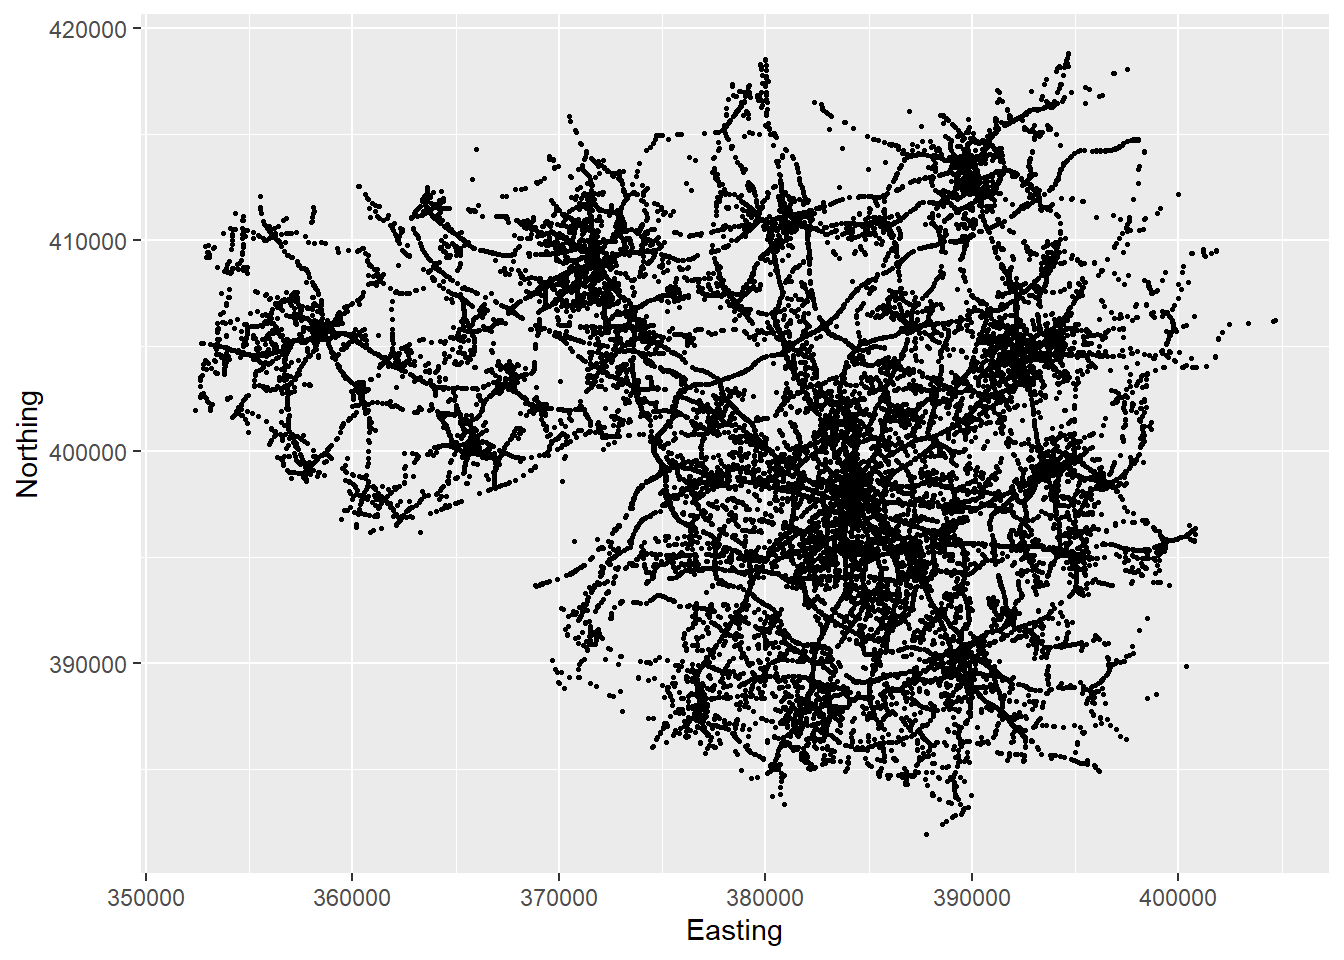
\includegraphics{R_FirstSteps_files/figure-latex/unnamed-chunk-36-1.pdf}

You can basically see where in Manchester accidents happened. In essence
you can see the Manchester Road network. The next image adds a few
flourishes to the picture.

\begin{Shaded}
\begin{Highlighting}[]
\FunctionTok{ggplot}\NormalTok{(accdata, }\FunctionTok{aes}\NormalTok{(}\AttributeTok{x =}\NormalTok{ Easting, }\AttributeTok{y=}\NormalTok{Northing,}\AttributeTok{color =}\NormalTok{ Road1Class)) }\SpecialCharTok{+} 
  \FunctionTok{geom\_point}\NormalTok{(}\AttributeTok{size=}\FloatTok{0.5}\NormalTok{) }\SpecialCharTok{+}
  \FunctionTok{ggtitle}\NormalTok{(}\StringTok{"Locations of vehicle accidents in Greater Manchester"}\NormalTok{)}
\end{Highlighting}
\end{Shaded}

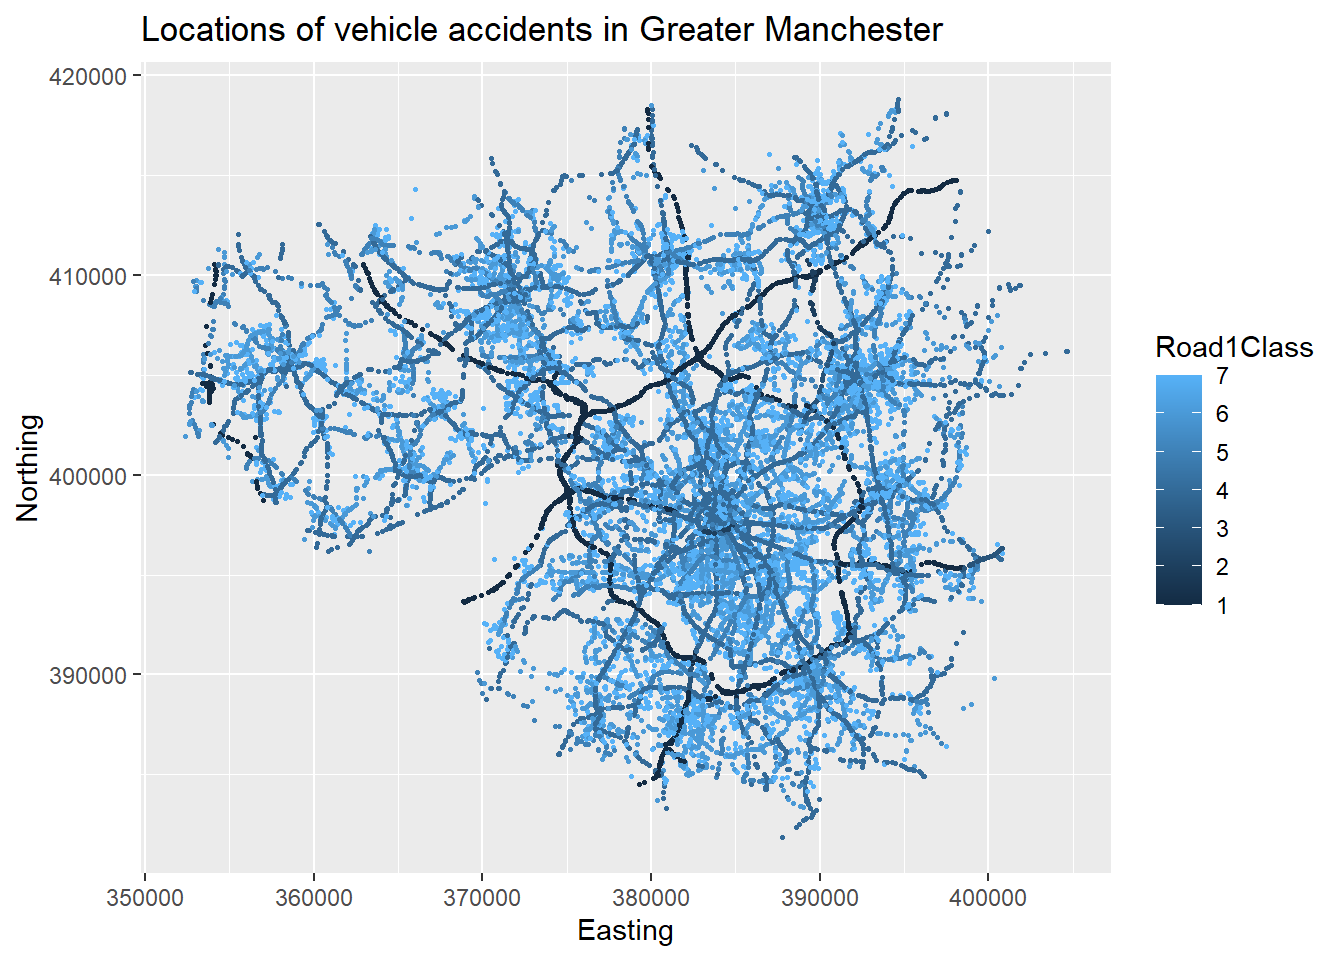
\includegraphics{R_FirstSteps_files/figure-latex/unnamed-chunk-37-1.pdf}

\hypertarget{end-of-session}{%
\section{End of session}\label{end-of-session}}

Before you leave RStudio you need to save your script file. That means
that tomorrow you can just come back open the script file and continue
to work.

\end{document}
